\wrapfSimple{ml/pca-maths/pca-maths-1}
We now show that among all possible linear dimensionality reduction method, PCA is optimal in sense of $\ell^2$ error. 
%
To simplify, without loss of generality (since it can be subtracted from the data) we assume that empirical mean is zero $\hat m=0$ so that $X=\tilde X$. 

We recall that $X=\sqrt{n} U \diag(\si) V^\top$ and $\hat C = \frac{1}{n} X^\top X = U \La U^\top$ where $\La = \diag(\la_i=\si_i^2)$, where $\la_1 \geq \ldots \geq \la_r$.  

\wrapfSimple{ml/pca-maths/pca-maths-2}
The following proposition shows that PCA is optimal in term of $\ell^2$ distance if one consider only affine spaces. This means that we consider the following compression/decompression to a dimension $k$ (i.e. dimensionality reduction and then expansion) 
\eql{\label{eq-pca-nonconvex}
	\umin{R,S} \enscond{
		f(R,S) \eqdef \sum_i \norm{x_i-R S^\top x_i}_{\RR^p}^2
		}{ R,S \in \RR^{p \times k} }
}
Note that this minimization is a priori not trivial to solve because, although $f(\cdot,S)$ and $f(R,\cdot)$ are convex, $f$ is not jointly convex. So iteratively minimizing on $R$ and $S$ might fail to converge to a global minimizer.
%
This section aims at proving the following theorem.

\begin{thm}\label{thm-pca-optim}
	A solution of~\eqref{eq-pca-nonconvex} is $S=R=V_{1:k} \eqdef [v_1,\ldots,v_k]$.
\end{thm}

Note that using such a compressor $R$ and decompressor $R=S$ corresponds exactly to the PCA method~\eqref{eq-pca-1} and~\eqref{eq-pca-2}.

We first prove that one can restrain its attention to orthogonal projection matrix.

\begin{lem}
	One can assume $S=R$ and $S^\top S = \Id_{k\times k}$.
\end{lem}
\begin{proof}
	We consider an arbitrary pair $(R,S)$. Since the matrix $R S^\top$ has rank $k' \leq k$, let $W \in \RR^{p \times k'}$ be an ortho-basis of $\Im(RS^\top)$, so that $W^\top W = \Id_{k' \times k'}$. We remark that 
	\eq{
		\uargmin{z} \norm{x-Wz}^2 = W^\top x
	}
	because the first order condition for this problem reads $W^\top(Wz-x)=0$.
	%	
	Hence, denoting $RS^\top x_i = Wz_i$ for some $z_i \in \RR^{k'}$
	\eq{
		f(R,S) = \sum_i \norm{x_i - RS^\top x_i}^2 = \sum_i \norm{x_i - W z_i}^2 \geq \sum_i \norm{x_i - W W^\top x_i}^2
		\geq  f(\tilde W,\tilde W).
	}
	were we have extended $W$ in an orthogonal matrix $\tilde W \in \RR^{p \times k}$ where $\tilde W_{1:k'}=W$.
\end{proof}

\begin{lem}
	Denoting $C \eqdef XX^\top \in \RR^{p \times p}$, an optimal $S$ is obtained by solving
	\eq{
		\umax{S \in \RR^{p \times k}} \enscond{\tr(S^\top C S^\top)}{ S^\top S=\Id_{k} }.
	}
\end{lem}
\begin{proof}
	Using the previous lemma, one can consider only $R=S$ with $S^\top S=\Id_{k}$ so that one needs to solve
	\eq{
		f(S,S) = \sum_i \norm{x_i SS^\top x_i}^2
		= \sum_i \norm{x_i}^2 - 2 x_i^\top S S^\top x_i + x_i^\top S(S^\top S) S^\top x_i.
	}
	Using that $S^\top S=\Id_k$, one has
	\eq{
		f(S,S) = \text{cst} - \sum_i x_i^\top S S^\top x_i
		= - \sum_i \tr(x_i^\top S S^\top x_i)
		= - \sum_i \tr(S^\top x_i x_i^\top S )
		= - \tr( S^\top (\sum_i x_i x_i^\top) S ).
	}
\end{proof}

The next lemma provides an upper bound on the quantity being minimized as the solution of a convex optimization problem (a linear program). The proof of the theorem follows by showing that this upper bound is actually reached, which provides a certificate of optimality.  

\begin{lem}\label{lem-upper-bound-pca}
	Denoting $C=V \La V^\top$, one has 
	\eql{\label{eq-variational-pca}
		\tr(S^\top C S) \leq \umax{\be \in \RR^p}
			\enscond{ \sum_{i=1}^p \la_i \be_i }{ 0 \leq \be \leq 1, \sum_i \be_i \leq k }
			= \sum_{i=1}^k \la_i
	}
	i.e. the maximum on the right hand size is $\be=(1,\ldots,1,0,\ldots,0)$.
\end{lem}
\begin{proof}
	We extend $V \in \RR^{p \times k}$ into an orthogonal matrix $\tilde V \in \RR^{p \times p}$ (i.e. $\tilde V_{1:r}=V$) such 
	that $\tilde V\tilde V^\top = \tilde V^\top V = \Id_p$. Similarly we extend $\La$ into $\tilde\La$ by adding zeros, so that $C=\tilde V \tilde \La \tilde V^\top$.  One has
	\eq{
		\tr(S^\top C S) = \tr(S^\top \tilde V \tilde \La \tilde V^\top S)
		= \tr(B^\top \La B) = \tr(\La BB^\top) = \sum_{i=1}^p \la_i \norm{b_i}^2
		= \sum_i \la_i \be_i
	}
	where we denoted $B \eqdef V^\top S \in \RR^{p \times k}$, $(b_i)_{i=1}^p$ with $b_i \in \RR^k$ are the rows of $B$ and $\be_i \eqdef \norm{b_i}^2 \geq 0$.
	%
	One has
	\eq{
		B^\top B = S^\top \tilde V \tilde V^\top S = S^\top S = \Id_k, 
	}
	so that the columns of $B$ are orthogonal, and thus
	\eq{
		\sum_i \be_i = \sum_i \norm{b_i}^2 = \norm{B}_{\text{Fro}}^2 = \tr(B^\top B) = \tr(B^\top B) = k.
	}		
	
	\begin{figure}
\centering
\begin{tabular}{@{}c@{\hspace{10mm}}c@{\hspace{10mm}}c@{}}
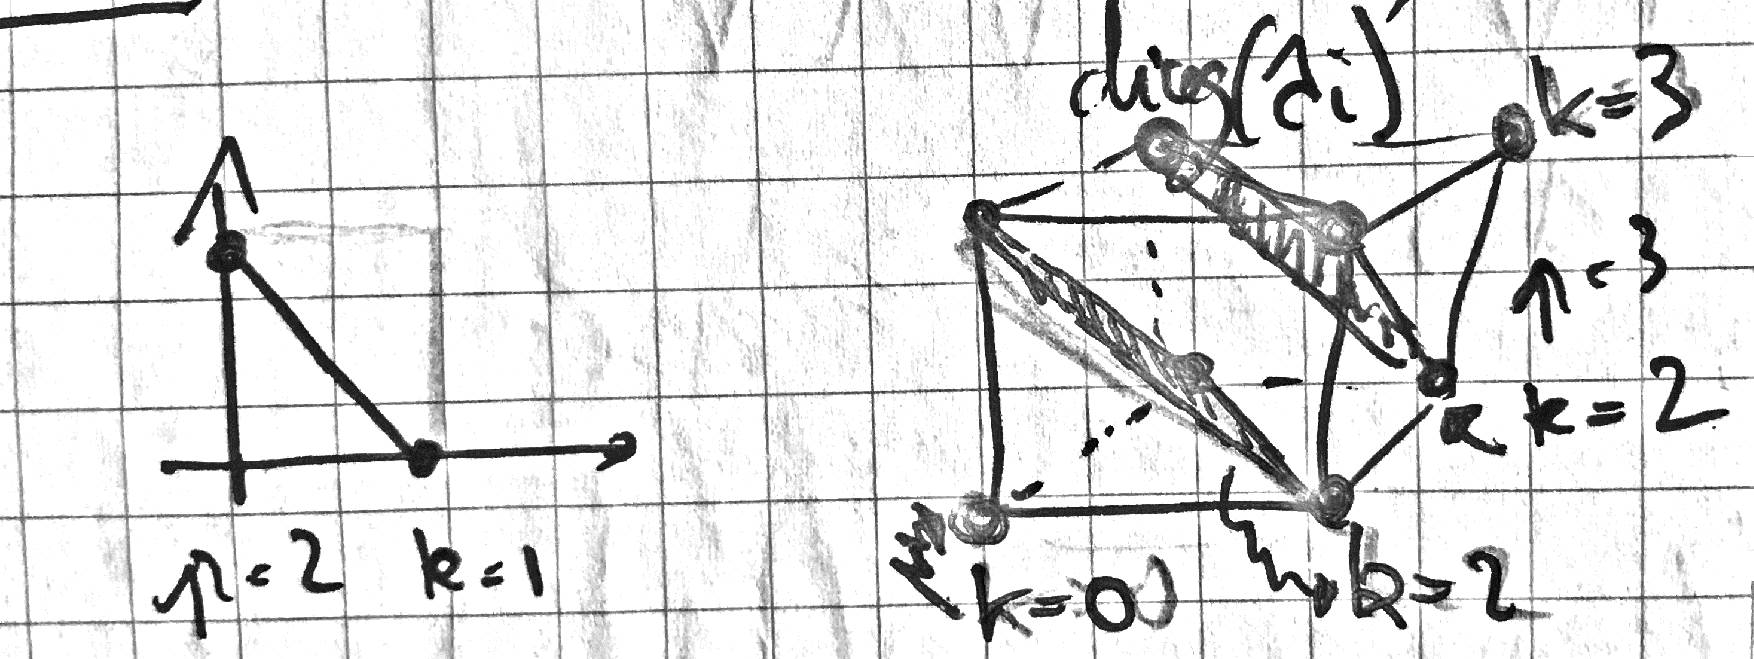
\includegraphics[width=.3\linewidth]{ml/pca-maths/pca-maths-3}&
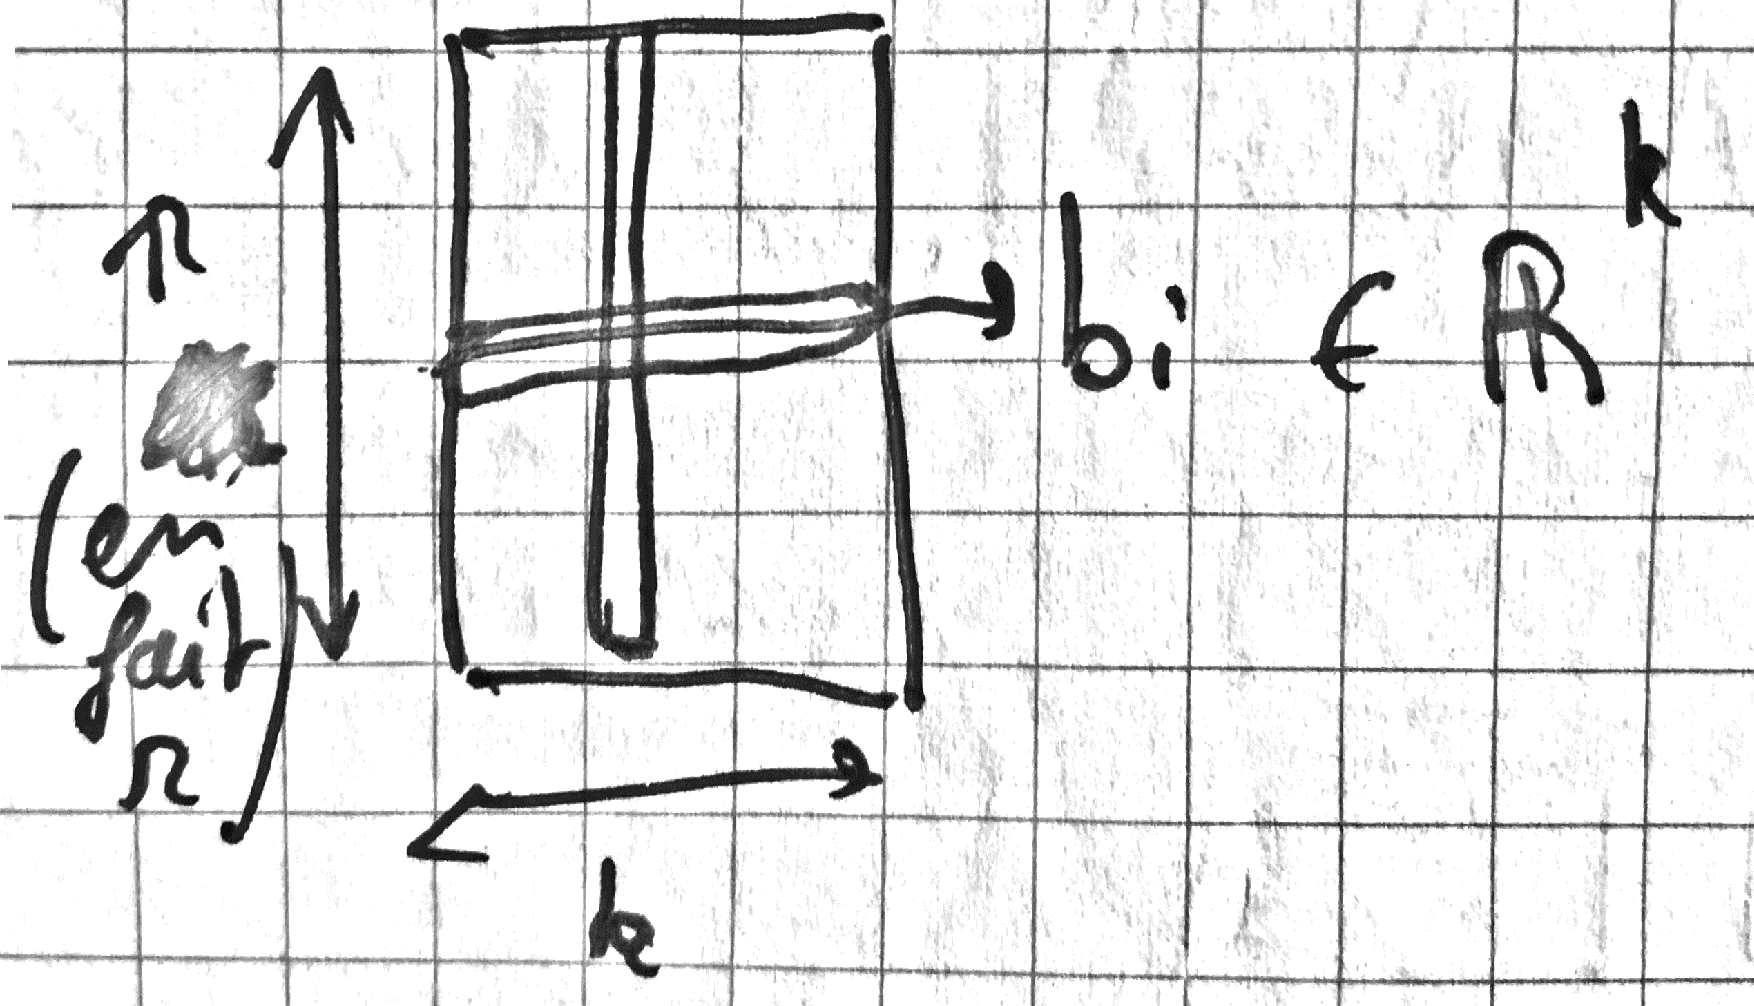
\includegraphics[width=.2\linewidth]{ml/pca-maths/pca-maths-4}&
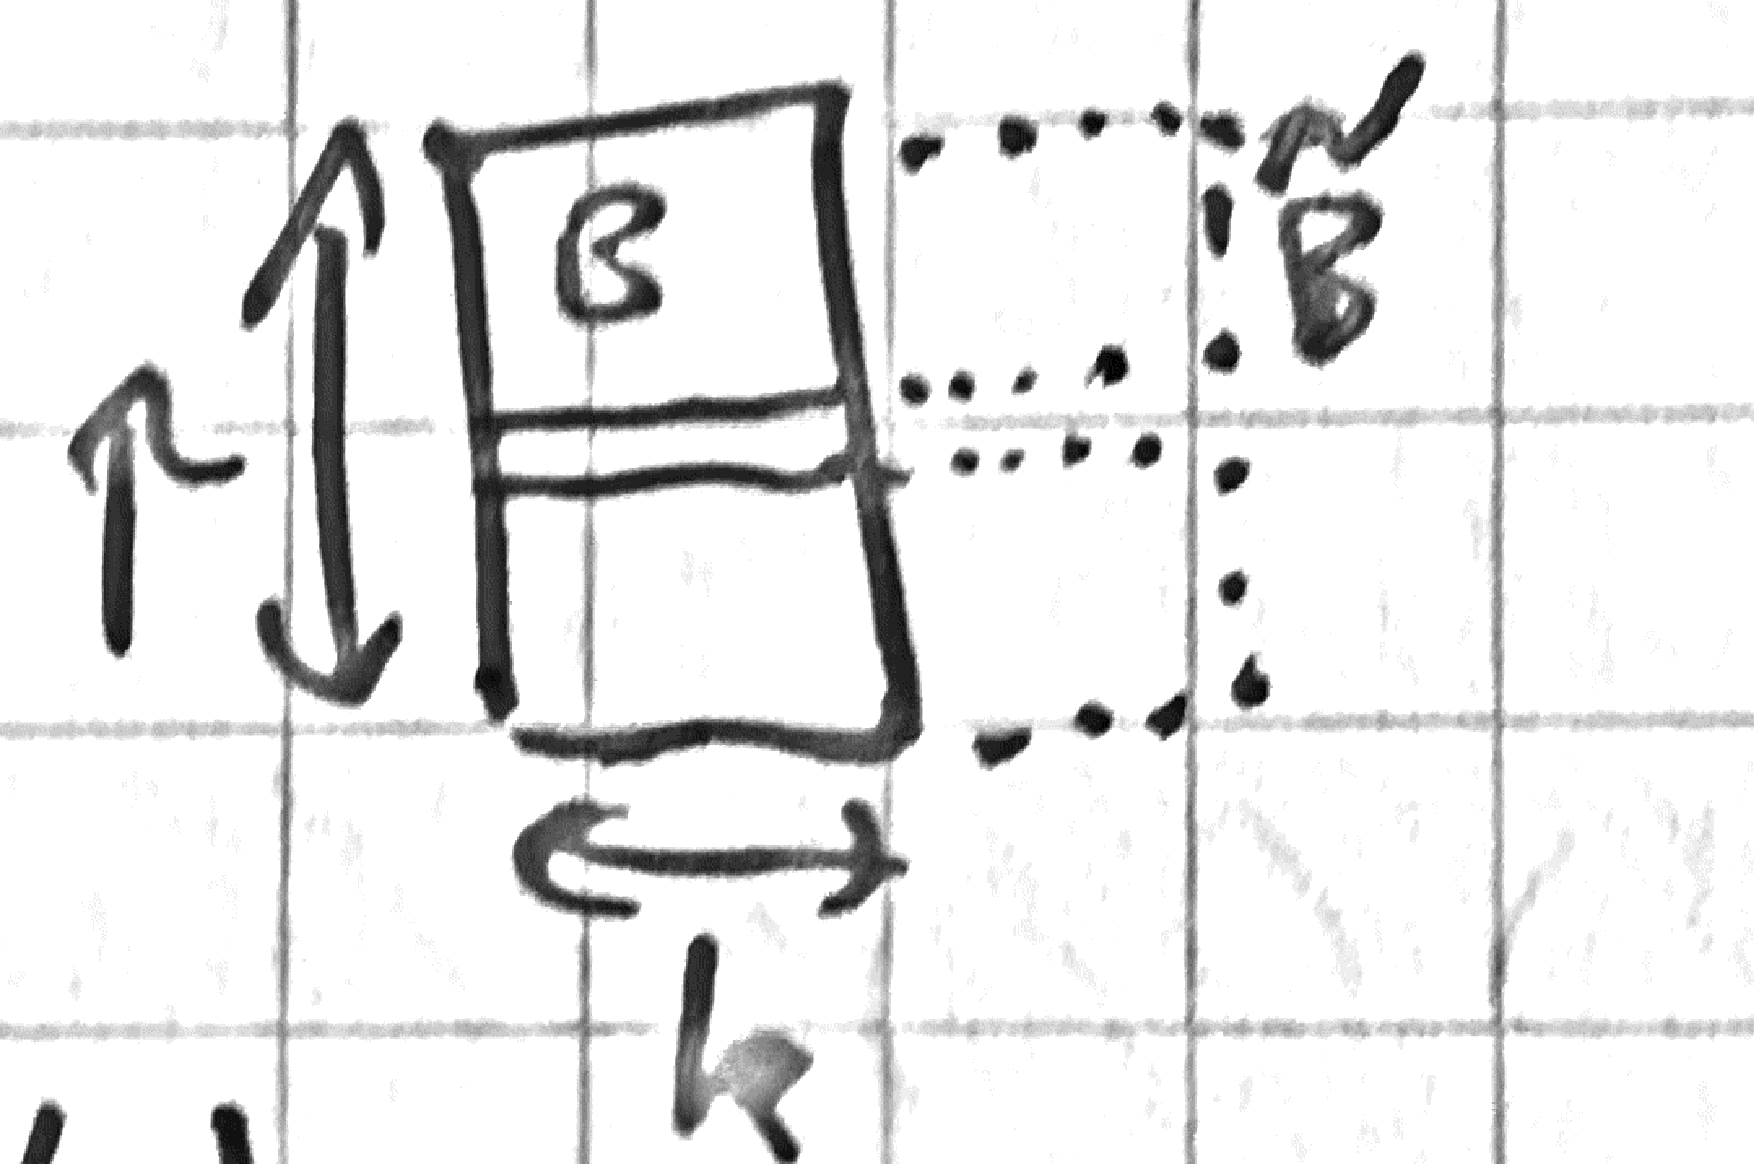
\includegraphics[width=.2\linewidth]{ml/pca-maths/pca-maths-5}
\end{tabular}
\caption{\label{fig-pca-var-proof}
Left: proof of the rightmost inequality in~\eqref{eq-variational-pca}. Middle: matrix $B$, right: matrix $\tilde B$. 
}
\end{figure}


	We extend the $k$ columns of $b$ into an orthogonal basis $\tilde B \in \RR^{p \times p}$ such that $\tilde B \tilde B^\top = \tilde B^\top \tilde = \Id_p$, so that 
	\eq{
		0 \leq \be_i = \norm{b_i}^2 \leq \norm{\tilde b_i}^2 = 1
	}
	and hence $(\be_i)_{i=1}^p$ satisfies the constraint of the considered optimization problem, hence $\tr(S^\top C S)$ 
	is necessarily smaller than the maximum possible value. 
	%
	
	For the proof of the second upper bound, we only verify it in 2D and 3D using a drawing, see Figure~\ref{fig-pca-var-proof}, left. 
\end{proof}

\begin{proof}[Proof of Theorem~\ref{thm-pca-optim}]
	Setting $S=V_{1:k}=[v_1,\ldots,v_k]$, it satisfies $CS = V \La V^\top V_{1:k} = V_{1:k} \diag(\la_i)_{i=1}^k$ and hence
	\eq{
		\tr(S^\top C S) = \tr(S^\top S \diag(\la_i)_{i=1^k}) = \tr(\Id_k \diag(\la_i)_{i=1^k}) = \sum_{i=1}^k \la_i.
	}
	This value matches the right-most upper bound of Lemma~\ref{lem-upper-bound-pca}, which shows that this $S$ is optimal.
\end{proof}


%\begin{prop}
%	One has
%	\eq{
%		(\tilde x,\tilde T) \in \uargmin{ (\bar x,\bar T) } \enscond{ \sum_i \norm{x_i - \bar x_i }^2 }{ \foralls i, \bar x_i \in \bar T }
%	}
%	where $\bar T$ is constrained to be a $d$-dimensional affine space. 
%\end{prop}
